\apendice{Especificación de Requisitos}

\section{Introducción}\label{intoduccion-requisitos}

Este anexo recoge la especificación de requisitos que define el comportamiento del sistema desarrollado. Se han seguido las recomendaciones del estándar IEEE 830-1998 \cite{ieee}, que establece que una buena especificación de requisitos software debe ser:

\begin{itemize}
    \item \textbf{Completa:} Todos los requerimientos deben estar incluidos y todas las referencias definidas.
    \item \textbf{Consistente:} Debe ser coherente tanto internamente como con otros documentos de especificación.
    \item \textbf{Inequívoca:} La redacción debe ser clara para evitar malentendidos.
    \item \textbf{Correcta:} El software debe cumplir con los requisitos especificados.
    \item \textbf{Trazable:} Debe ser posible rastrear la historia, ubicación o aplicación de un ítem a través de su identificación documentada.
    \item \textbf{Priorizable:} Los requisitos deben poder organizarse jerárquicamente según su relevancia para el negocio, clasificándolos en esenciales, condicionales y opcionales.
    \item \textbf{Modificable:} Los requerimientos deben ser fácilmente modificables.
    \item \textbf{Verificable:} Debe existir un método finito y sin costo para probar los requisitos.
\end{itemize}

\section{Objetivos generales}\label{objetivos-generales}

El proyecto tiene los siguientes objetivos generales.

\begin{itemize}
    \item Demostrar empíricamente que al aplicar métodos de transformación invariante de la iluminación, se consiguen mejores resultados a la hora de identificar piezas metálicas mediante métodos de agrupamiento de imágenes.
    \item Desarrollar una aplicación de escritorio que tome como entrada una imagen y  permita al usuario evaluar los resultados de la segmentación para la identificación de piezas metálicas. La aplicación debe ofrecer diferentes algoritmos tanto de transformación invariante (propuestos por Álvarez \cite{alvarez2011}, Maddern \cite{maddern2014}, Krajník \cite{krajník2015}, Upcroft \cite{upcroft2014} y PCA \cite{pca2017}) como de agrupamiento de imágenes (K-Means \cite{MATLAB:2023bKmeans}, Fuzzy C-Means \cite{MATLAB:2023bFuzzy}, GMM \cite{MATLAB:2023bGMM} y agrupamiento con información espacial \cite{wang2012hmrf}).
    \item Desarrollar una aplicación de escritorio que permita evaluar la mejora que supone la aplicación de los métodos de transformación invariante en procesos de segmentación de imágenes, mostrando una comparación de los resultados tanto visual como numérica.
    \item Guardar las imágenes resultantes del método de transformación invariante y las dos imágenes  resultados de la segmentación, una aplicando la transformación de invariantes de iluminación y otra aplicando la segmentación directamente a la imagen original.
    \item Comparar los resultados de distintos métodos de transformación invariante de imágenes y argumentar la mejora que se obtiene en la identificación de piezas metálicas.
\end{itemize}

\section{Catálogo de requisitos}\label{catalogo-de-requisitos}

En este apartado se enumeran los requisitos específicos que se derivan de los objetivos generales del proyecto.

\subsection{Requisitos funcionales}\label{requisitos-funcionales}

A continuación, se enumerarán los requisitos funcionales.

\begin{itemize}
    \item \textbf{RF-1 Gestión de transformación invariante:} La aplicación debe ser capaz de gestionar la transformación invariante sobre imágenes.
    \begin{itemize}
        \item \textbf{RF-1.1 Seleccionar imagen:} El usuario debe poder seleccionar una imagen sobre la cual aplicar las diferentes transformaciones.
        \begin{itemize}
            \item \textbf{RF-1.1.1 Imagen del sistema:} El usuario debe poder seleccionar una imagen de prueba contenida en el programa.
            \begin{itemize}
                \item \textbf{RF-1.1.1.1 Carga automática de la imagen ground truth:} Al haber seleccionado una imagen contenida en el programa, esta tendrá asociada una imagen ground truth.
            \end{itemize}
            \item \textbf{RF-1.1.2 Imagen propia del usuario:} El usuario debe poder seleccionar una imagen propia. Al no tener imagen ground truth asociada esta no se cargará automáticamente.
            \begin{itemize}
                \item \textbf{RF-1.1.2.1 Seleccionar una imagen ground truth propia:} Debido a que la imagen que el usuario ha seleccionado es una imagen propia, el sistema permitirá aportar su correspondiente imagen ground truth.
                \item \textbf{RF-1.1.2.2 Modificar imagen ground truth seleccionada:} El usuario debe poder modificar la imagen ground truth proporcionada en el caso de que se haya seleccionado una imagen propia.
            \end{itemize}
            \item \textbf{RF-1.1.3 Modificar imagen seleccionada:} El usuario debe poder seleccionar una imagen diferente a la seleccionada anteriormente sobre la cual aplicar las diferentes transformaciones.
        \end{itemize}
        \item \textbf{RF-1.2 Seleccionar algoritmo invariante:} El usuario debe poder seleccionar el algoritmo de transformación invariante que desee de la lista de algoritmos que la aplicación ofrece.
        \item \textbf{RF-1.3 Seleccionar algoritmo de agrupamiento:} El usuario debe poder seleccionar el algoritmo de agrupamiento invariante que desee de la lista de algoritmos que la aplicación ofrece.
        \item \textbf{RF-1.4 Seleccionar número de centros:} El usuario debe poder seleccionar el numero de centros que desee como parámetro del algoritmo de agrupamiento seleccionado dentro de unos limites preestablecidos.
        \item \textbf{RF-1.5 Almacenar resultados en caché:} La aplicación debe guardar en caché los resultados de la ejecución.
        \item \textbf{RF-1.6 Recuperar resultados almacenados en caché:} La aplicación recuperar los resultados de antiguas ejecuciones con los mismos parámetros para ahorrar costes computacionales.
        \item \textbf{RF-1.7 Guardar imágenes resultantes:} El usuario debe poder guardar los resultados de la ejecución en el directorio que desee.
    \end{itemize}
    \item \textbf{RF-2 Gestión de caché:} La aplicación debe ser capaz de gestionar correctamente una memoria caché donde almacenar y mostrar los resultados de as ejecuciones del usuario.
    \begin{itemize}
        \item \textbf{RF-2.1 Visualizar información de antiguas ejecuciones en formato tabla:} La aplicación debe mostrar en una tabla una lista de los resultados de las distintas ejecuciones almacenadas en caché.
        \begin{itemize}
            \item \textbf{RF-2.1.1 Poder reordenar las columnas:} El usuario debe poder reordenar la tabla de la caché en función de los datos contenidos en las diferentes columnas.
            \item \textbf{RF-2.1.2 Visualizar la imagen correspondiente a la fila seleccionada:} El usuario debe poder acceder en especifico a la imagen a la que hace alusión cada fila de la tabla caché.
        \end{itemize}
        \item \textbf{RF-2.2 Abrir el directorio de la caché:} El usuario debe poder acceder al directorio de la caché.
        \item \textbf{RF-2.3 Borrar contenido de la caché:} El usuario debe poder borrar el contenido de la caché.
    \end{itemize}
    \item \textbf{RF-3 Configuración:} El usuario debe poder configurar los parámetros disponibles de la aplicación. 
    \begin{itemize}
        \item \textbf{RF-3.1 Seleccionar el idioma:} El usuario debe poder seleccionar el idioma de la aplicación dependiendo si desea trabajar con esta en español o en inglés. 
    \end{itemize}
    \item \textbf{RF-4 Ayuda:} El usuario debe poder obtener ayuda sobre los distintos elementos de la aplicación.
    \begin{itemize}
        \item \textbf{RF-4.1 Documentación dentro de la aplicación:} La aplicación debe contener distintos apartados dedicados a documentar el funcionamiento y métodos aplicados en la aplicación. 
        \item \textbf{RF-4.2 Tooltips:} La aplicación debe proporcionar información sobre la funcionalidad de las distintas acciones dentro de esta.
    \end{itemize}
\end{itemize}

\subsection{Requisitos no funcionales}\label{requisitos-no-funcionales}

A continuación, se enumerarán los requisitos no funcionales.

\begin{itemize}
    \item \textbf{RNF-1 Usabilidad:} La aplicación debe tener una interfaz de usuario intuitiva y fácil de usar, con una curva de aprendizaje mínima.
    \item \textbf{RNF-2 Mensajes de error explicativos:} La aplicación debe proporcionar mensajes de error claros y explicativos que ayuden al usuario a entender y resolver el problema.
    \item \textbf{RNF-3 Rendimiento:} La aplicación debe tener unos tiempos de carga aceptables.
    \item \textbf{RNF-4 Disponibilidad:} La aplicación debe estar preparada para funcionar en cualquier localización y sin acceso a internet.
    \item \textbf{RNF-5 Soporte:} La aplicación debe dar soporte a versiones de iguales o superiores a MATLAB 2023b.
    \item \textbf{RNF-6 Uso de recursos:} La aplicación debe ser eficiente en el uso de recursos del sistema, reutilizando los resultados de ejecuciones anteriores para reducir costes computacionales.
    \item \textbf{RNF-7 Modularidad:} La aplicación debe estar diseñada de manera modular, permitiendo la fácil adición o modificación de funcionalidades sin afectar otras partes del sistema.
    \item \textbf{RNF-8 Internacionalización:} La aplicación debe estar preparada para soportar varios idiomas.
    \item \textbf{RNF-9 Compatibilidad:} La aplicación debe poderse ejecutar en distintos sistemas operativos. Por lo menos en Linux y en Windows.
\end{itemize}

\section{Especificación de requisitos}\label{especificación-de-requisitos}

En esta sección se mostrará el diagrama de casos de uso resultante de los requisitos funcionales y se desarrollará cada uno de ellos.

\subsection{Diagrama de casos de uso}\label{diagrama-de-casos-de-uso}

A continuación, se muestra en la figura \ref{fig:Diagrama_de_casos_de_uso} el diagrama de casos de uso.

\begin{figure}[!h]
    \centering
    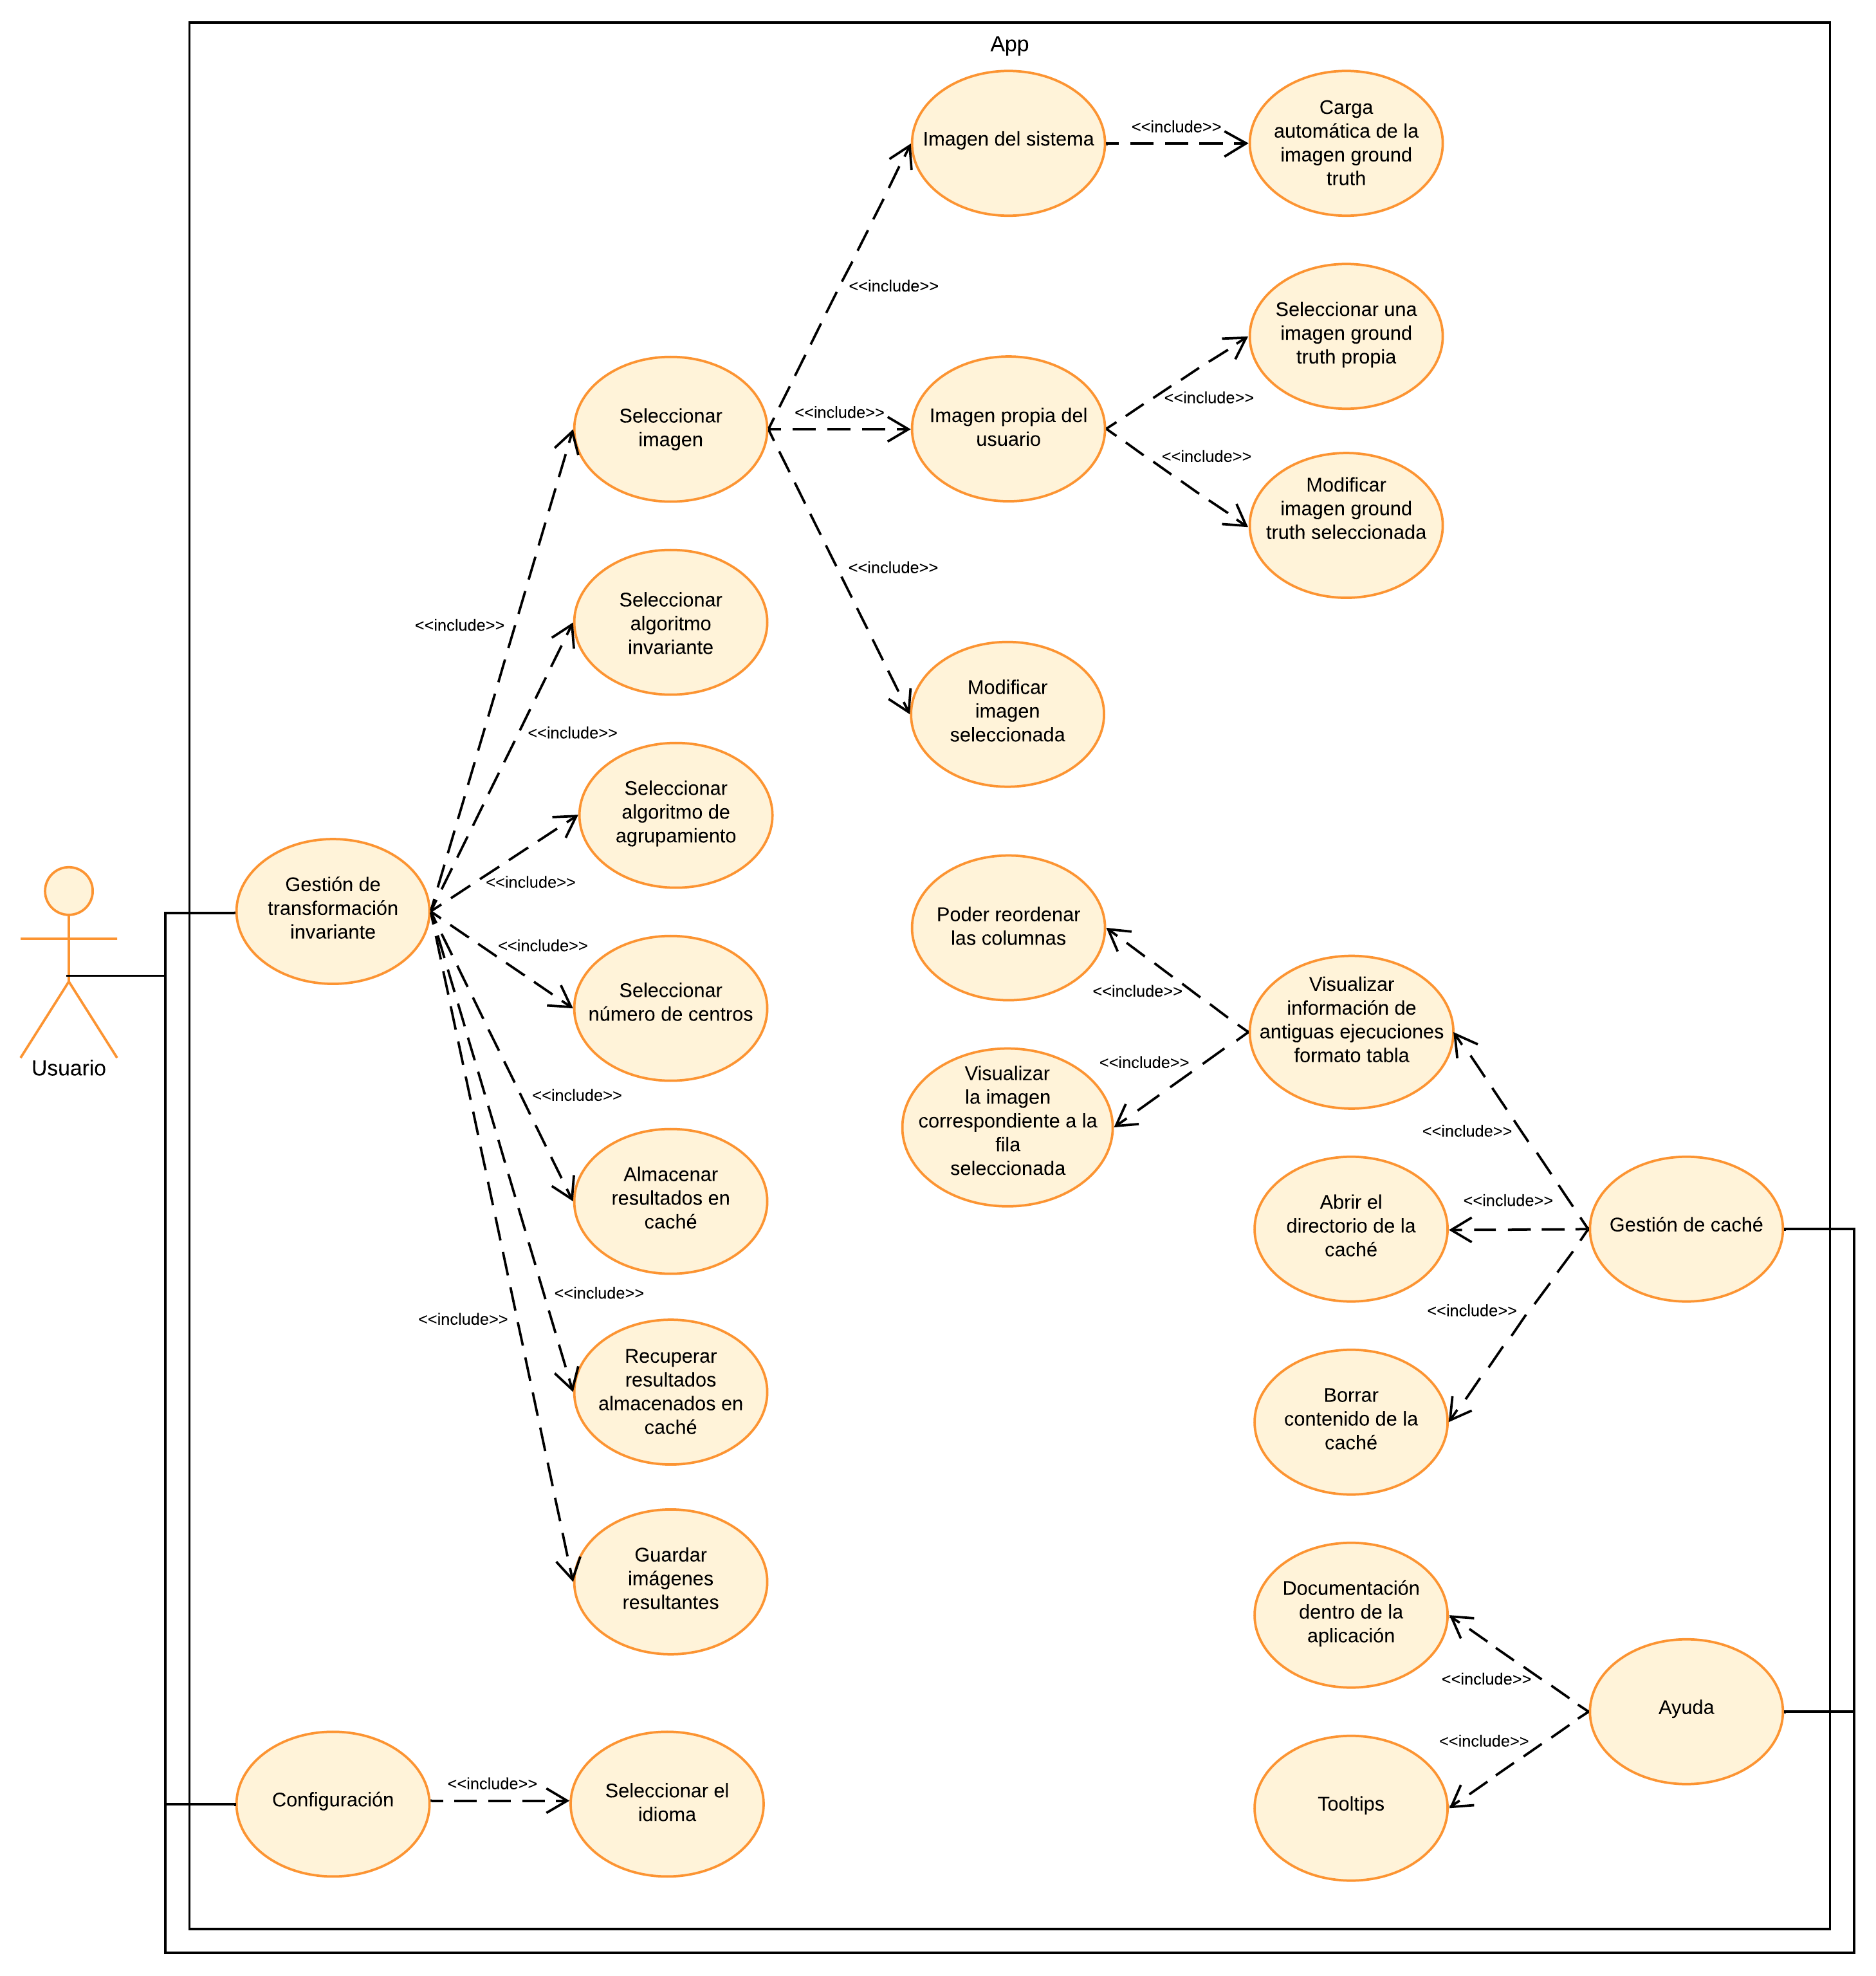
\includegraphics[width=1\textwidth]{Diagrama_de_casos_de_uso}
    \caption{Diagrama de casos de uso de la aplicación InvIPM.}\label{fig:Diagrama_de_casos_de_uso}
\end{figure}

\newpage

\subsection{Actores}\label{actores}

El sistema está diseñado para la interacción de un único actor, identificado como el usuario. Este usuario idealmente será personal especializado en el análisis de la calidad de piezas metálicas a través de imágenes, generalmente asociado a una empresa. No obstante, la aplicación ha sido desarrollada con la capacidad de instruir a usuarios que no posean los conocimientos necesarios, a través de una documentación integrada y accesible dentro de la propia aplicación.

\subsection{Casos de uso}\label{casos-de-uso}

A continuación, se definirán los casos de uso.

\begin{table}[p]
	\centering
	\begin{tabularx}{\linewidth}{ p{0.21\columnwidth} p{0.71\columnwidth} }
		\toprule
		\textbf{CU-1}    & \textbf{Gestión de transformación invariante}\\
		\toprule
		\textbf{Versión}              & 1.0    \\
		\textbf{Autor}                & Jonás Martínez Sanllorente \\
		\textbf{Requisitos asociados} & RF-1, RF-1.1, RF-1.1.1, RF-1.1.1.1, RF-1.1.2, RF-1.1.2.1, RF-1.1.2.2, RF-1.1.3, RF-1.2, RF-1.3, RF-1.4, RF-1.5, RF-1.6, RF-1.7 \\
		\textbf{Descripción}          & Permite al usuario aplicar sobre una imagen los distintos métodos de transformación invariante y guardar los resultados.\\
		\textbf{Precondición}         & La aplicación se encuentra disponible \\
		\textbf{Acciones}             &
		\begin{enumerate}
			\def\labelenumi{\arabic{enumi}.}
			\tightlist
			\item El usuario pulsa en la pestaña de exploración de algoritmos
            \item El usuario selecciona una imagen de pieza metálica.
            \item El usuario selecciona un algoritmo de transformación invariante.
            \item El usuario selecciona un algoritmo de agrupamiento.
            \item El usuario selecciona un numero de centros (por defecto 2).
            \item El usuario hace click en el botón de ejecutar.
            \item El programa ejecuta sobre la imagen seleccionada el algoritmo invariante seleccionado y mas tarde el algoritmo de agrupamiento sobre la original y sobre la invariante.
            \item En el caso de que tenga imagen ground truth calcula el porcentaje de acierto.
            \item El programa guarda en la cache los resultados.
            \item El programa muestra cuatro imágenes tras finalizarse la ejecución:
            \begin{itemize}
                \item Imagen original.
                \item Imagen original segmentada.
                \item Imagen invariante.
                \item Imagen invariante segmentada.
            \end{itemize}
            \item El usuario hace click en el botón de guardar resultados y selecciona un directorio donde guardar las imágenes.
		\end{enumerate}\\
		\textbf{Postcondición}        & Se muestran los resultados de la transformación invariante y las segmentaciones indicando en el caso de que haya imagen ground truth la tasa de acierto.\\
		\textbf{Excepciones}          & Error (mensaje) \\
		\textbf{Importancia}          & Alta \\
		\bottomrule
	\end{tabularx}
	\caption{CU-1 Gestión de transformación invariante.}
\end{table}

\begin{table}[p]
	\centering
	\begin{tabularx}{\linewidth}{ p{0.21\columnwidth} p{0.71\columnwidth} }
		\toprule
		\textbf{CU-2}    & \textbf{Seleccionar imagen}\\
		\toprule
		\textbf{Versión}              & 1.0    \\
		\textbf{Autor}                & Jonás Martínez Sanllorente \\
		\textbf{Requisitos asociados} & RF-1.1, RF-1.1.1, RF-1.1.1.1, RF-1.1.2, RF-1.1.2.1, RF-1.1.2.2, RF-1.1.3 \\
		\textbf{Descripción}          & Permite al usuario seleccionar una imagen sobre la que aplicar los distintos métodos de transformación invariante.\\
		\textbf{Precondición}         & La aplicación se encuentra disponible \\
		\textbf{Acciones}             &
		\begin{enumerate}
			\def\labelenumi{\arabic{enumi}.}
			\tightlist
			\item El usuario pulsa en la pestaña de exploración de algoritmos
            \item El usuario hace click en el botón de cargar imagen de pieza metálica.
            \item Se muestra el directorio de imágenes del programa.
            \item El usuario selecciona una imagen del programa o propia.
            \item El usuario hace click en el botón de aceptar.
            \begin{itemize}
                \item En el caso de seleccionar una imagen del programa, la aplicación busca su correspondiente imagen ground truth.
                \item En el caso de seleccionar una imagen propia, se notifica al usuario de que al no ser una imagen del programa esta no tiene imagen ground truth asociada.
            \end{itemize}
            \item Si no hay ningún error: Se guardan en memoria la imagen y se muestra en sus correspondiente plot y si es una imagen del programa también la imagen ground truth.
		\end{enumerate}\\
		\textbf{Postcondición}        & 
           \begin{enumerate}
                \item La imagen seleccionada se ha cargado correctamente.
                \item Activa la interacción de los selectores de método invariante, método de agrupamiento, numero de centro y el botón de ejecutar.
            \end{enumerate}\\
		\textbf{Excepciones}          & Se ha cancelado la selección de imágenes. (mensaje).\newline
                                        Image selection has been canceled. (mensaje).\newline
                                        Imagen ground truth no encontrada. (mensaje).\newline
                                        Ground truth image not found (mensaje). \\
		\textbf{Importancia}          & Alta \\
		\bottomrule
	\end{tabularx}
	\caption{CU-2 Seleccionar imagen.}
\end{table}

\begin{table}[p]
	\centering
	\begin{tabularx}{\linewidth}{ p{0.21\columnwidth} p{0.71\columnwidth} }
		\toprule
		\textbf{CU-3}    & \textbf{Imagen del sistema}\\
		\toprule
		\textbf{Versión}              & 1.0    \\
		\textbf{Autor}                & Jonás Martínez Sanllorente \\
		\textbf{Requisitos asociados} & RF-1.1.1, RF-1.1.1.1 \\
		\textbf{Descripción}          & El usuario debe poder seleccionar una imagen de prueba contenida en el programa \\
		\textbf{Precondición}         & La aplicación se encuentra disponible.\newline
                                        El usuario ha hecho click en el botón de cargar imagen de pieza metálica.\\
		\textbf{Acciones}             &
		\begin{enumerate}
			\def\labelenumi{\arabic{enumi}.}
			\tightlist
			\item El usuario selecciona una imagen de las proporcionadas por el sistema.
			\item La aplicación carga la imagen seleccionada.
            \item La aplicación busca la imagen ground truth correspondiente a la imagen seleccionada.
            \item Si no hay ningún error se muestra la imagen y su correspondiente imagen ground truth.
		\end{enumerate}\\
		\textbf{Postcondición}        & La imagen seleccionada se ha cargado correctamente. \\
		\textbf{Excepciones}          & Se ha cancelado la selección de imágenes. (mensaje).\newline
                                        Image selection has been canceled. (mensaje).\newline
                                        Imagen ground truth no encontrada. (mensaje).\newline
                                        Ground truth image not found (mensaje). \\
		\textbf{Importancia}          & Alta \\
		\bottomrule
	\end{tabularx}
	\caption{CU-3 Imagen del sistema.}
\end{table}

\begin{table}[p]
	\centering
	\begin{tabularx}{\linewidth}{ p{0.21\columnwidth} p{0.71\columnwidth} }
		\toprule
		\textbf{CU-4}    & \textbf{Carga automática de la imagen ground truth}\\
		\toprule
		\textbf{Versión}              & 1.0    \\
		\textbf{Autor}                & Jonás Martínez Sanllorente \\
		\textbf{Requisitos asociados} & RF-1.1.1.1 \\
		\textbf{Descripción}          & Al haber seleccionado una imagen de la aplicación, se cargara su correspondiente imagen ground truth.\\
		\textbf{Precondición}         & La aplicación se encuentra disponible.\newline
                                        El usuario ha hecho click en el botón de cargar imagen de pieza metálica.\newline
                                        El usuario ha seleccionado una imagen del sistema. \\
		\textbf{Acciones}             &
		\begin{enumerate}
			\def\labelenumi{\arabic{enumi}.}
			\tightlist
			\item La aplicación busca la correspondiente imagen ground truth de la imagen seleccionada en el directorio de imágenes ground truth.
			\item Si no hay ningún error se muestra la imagen ground truth en el plot correspondiente.
		\end{enumerate}\\
		\textbf{Postcondición}        & Imagen ground truth se ha cargado correctamente. \\
		\textbf{Excepciones}          & Imagen ground truth no encontrada. (mensaje).\newline
                                        Ground truth image not found (mensaje). \\
		\textbf{Importancia}          & Media. \\
		\bottomrule
	\end{tabularx}
	\caption{CU-4 Carga automática de la imagen ground truth.}
\end{table}

\begin{table}[p]
	\centering
	\begin{tabularx}{\linewidth}{ p{0.21\columnwidth} p{0.71\columnwidth} }
		\toprule
		\textbf{CU-5}    & \textbf{Imagen propia del usuario}\\
		\toprule
		\textbf{Versión}              & 1.0    \\
		\textbf{Autor}                & Jonás Martínez Sanllorente \\
		\textbf{Requisitos asociados} & RF-1.1.2, RF-1.1.2.1, RF-1.1.2.2 \\
		\textbf{Descripción}          & El usuario debe poder seleccionar una imagen propia. \\
		\textbf{Precondición}         & La aplicación se encuentra disponible.\newline
                                        El usuario ha hecho click en el botón de cargar imagen de pieza metálica. \\
		\textbf{Acciones}             &
		\begin{enumerate}
			\def\labelenumi{\arabic{enumi}.}
			\tightlist
			\item El usuario selecciona una imagen propia.
			\item La aplicación carga la imagen seleccionada.
            \item La aplicación busca informa al usuario que al ser una imagen propia, esta no tiene imagen ground truth asociada.
            \item Si no hay ningún error se muestra la imagen.
            \item La aplicación activa la interacción del botón de cargar una imagen ground truth propia.
		\end{enumerate}\\
		\textbf{Postcondición}        & La imagen seleccionada se ha cargado correctamente. \\
		\textbf{Excepciones}          & Se ha cancelado la selección de imágenes. (mensaje).\newline
                                        Image selection has been canceled. (mensaje).\newline
                                        Imagen ground truth no encontrada. (mensaje).\newline
                                        Ground truth image not found (mensaje). \\
		\textbf{Importancia}          & Alta \\
		\bottomrule
	\end{tabularx}
	\caption{CU-5 Imagen propia del usuario.}
\end{table}

\begin{table}[p]
	\centering
	\begin{tabularx}{\linewidth}{ p{0.21\columnwidth} p{0.71\columnwidth} }
		\toprule
		\textbf{CU-6}    & \textbf{Seleccionar una imagen ground truth propia}\\
		\toprule
		\textbf{Versión}              & 1.0    \\
		\textbf{Autor}                & Jonás Martínez Sanllorente \\
		\textbf{Requisitos asociados} & RF-1.1.2.1 \\
		\textbf{Descripción}          & La descripción del CU \\
		\textbf{Precondición}         & La aplicación se encuentra disponible.\newline
                                        El usuario ha cargado una imagen propia. \\
		\textbf{Acciones}             &
		\begin{enumerate}
			\def\labelenumi{\arabic{enumi}.}
			\tightlist
			\item El usuario hace click en el botón de cargar imagen ground truth.
			\item La aplicación abre un directorio para que el usuario seleccione el archivo que desee.
            \item El usuario selecciona la imagen que quiere utilizar como ground truth.
            \item Si no hay ningún error se muestra la imagen ground truth.
		\end{enumerate}\\
		\textbf{Postcondición}        & Imagen ground truth se ha cargado correctamente. \\
		\textbf{Excepciones}          & Error al leer la imagen ground truth: (mensaje).\newline
                                        Error reading ground truth image: (mensaje). \\
		\textbf{Importancia}          & Media \\
		\bottomrule
	\end{tabularx}
	\caption{CU-6 Seleccionar una imagen ground truth propia.}
\end{table}

\begin{table}[p]
	\centering
	\begin{tabularx}{\linewidth}{ p{0.21\columnwidth} p{0.71\columnwidth} }
		\toprule
		\textbf{CU-7}    & \textbf{Modificar imagen ground truth seleccionada}\\
		\toprule
		\textbf{Versión}              & 1.0    \\
		\textbf{Autor}                & Jonás Martínez Sanllorente \\
		\textbf{Requisitos asociados} & RF-1.1.2.2 \\
		\textbf{Descripción}          & El usuario debe poder modificar la imagen ground truth proporcionada en el caso de que se haya seleccionado una imagen propia. \\
		\textbf{Precondición}         & La aplicación se encuentra disponible.\newline
                                        El usuario ha cargado una imagen propia.\newline
                                        El usuario ha cargado una imagen ground truth propia.\\
		\textbf{Acciones}             &
		\begin{enumerate}
			\def\labelenumi{\arabic{enumi}.}
			\tightlist
			\item El usuario hace click en el botón de cargar imagen ground truth.
			\item La aplicación abre un directorio para que el usuario seleccione el archivo que desee.
            \item El usuario selecciona la imagen que quiere utilizar como ground truth.
            \item La aplicación elimina de memoria la imagen ground truth anterior y guarda en su lugar la nueva.
            \item Si no hay ningún error se muestra la imagen ground truth sustituyendo a la anterior.
		\end{enumerate}\\
		\textbf{Postcondición}        & Imagen ground truth nueva se ha cargado correctamente. \\
		\textbf{Excepciones}          & Error al leer la imagen ground truth: (mensaje).\newline
                                        Error reading ground truth image: (mensaje).\\
		\textbf{Importancia}          & Media \\
		\bottomrule
	\end{tabularx}
	\caption{CU-7 Modificar imagen ground truth seleccionada.}
\end{table}

\begin{table}[p]
	\centering
	\begin{tabularx}{\linewidth}{ p{0.21\columnwidth} p{0.71\columnwidth} }
		\toprule
		\textbf{CU-8}    & \textbf{Modificar imagen seleccionada}\\
		\toprule
		\textbf{Versión}              & 1.0    \\
		\textbf{Autor}                & Jonás Martínez Sanllorente \\
		\textbf{Requisitos asociados} & RF-1.1.3 \\
		\textbf{Descripción}          & El usuario debe poder seleccionar una imagen diferente a la seleccionada anteriormente \\
		\textbf{Precondición}         & La aplicación se encuentra disponible.\newline
                                        El usuario ha cargado una imagen anteriormente.\\
		\textbf{Acciones}             &
		\begin{enumerate}
			\def\labelenumi{\arabic{enumi}.}
			\tightlist
			\item El usuario hace click en el botón de cargar imagen de pieza metálica.
            \item Se muestra el directorio de imágenes del programa.
            \item El usuario selecciona una imagen del programa o propia.
            \item El usuario hace click en el botón de aceptar.
            \begin{itemize}
                \item En el caso de seleccionar una imagen del programa, la aplicación busca su correspondiente imagen ground truth.
                \item En el caso de seleccionar una imagen propia, se notifica al usuario de que al no ser una imagen del programa esta no tiene imagen ground truth asociada.
            \end{itemize}
            \item Si no hay ningún error se dejan de mostrar las imágenes tanto de entrada como de salida de anteriores ejecuciones, se boquea la interacción del botón de guardar resultados y: 
            \begin{itemize}
                \item En el caso de seleccionar una imagen del programa, se guardan en memoria tanto la imagen como la imagen ground truth y ambas se muestran en sus respectivos plots.
                \item En el caso de seleccionar una imagen propia, se guardan en memoria la imagen y se muestra en sus correspondiente plot.
            \end{itemize}
		\end{enumerate}\\
		\textbf{Postcondición}        & La imagen seleccionada se ha cargado correctamente. \\
		\textbf{Excepciones}          & Se ha cancelado la selección de imágenes. (mensaje).\newline
                                        Image selection has been canceled. (mensaje).\newline
                                        Imagen ground truth no encontrada. (mensaje).\newline
                                        Ground truth image not found (mensaje).\\
		\textbf{Importancia}          & Alta \\
		\bottomrule
	\end{tabularx}
	\caption{CU-8 Modificar imagen seleccionada.}
\end{table}

\begin{table}[p]
	\centering
	\begin{tabularx}{\linewidth}{ p{0.21\columnwidth} p{0.71\columnwidth} }
		\toprule
		\textbf{CU-9}    & \textbf{Seleccionar algoritmo invariante}\\
		\toprule
		\textbf{Versión}              & 1.0    \\
		\textbf{Autor}                & Jonás Martínez Sanllorente \\
		\textbf{Requisitos asociados} & RF-1.2 \\
		\textbf{Descripción}          & El usuario debe poder seleccionar el algoritmo de transformación invariante que desee de la lista de algoritmos que la aplicación ofrece. \\
		\textbf{Precondición}         & La aplicación se encuentra disponible.\newline
                                        El usuario ha cargado una imagen. \\
		\textbf{Acciones}             &
		\begin{enumerate}
			\def\labelenumi{\arabic{enumi}.}
			\tightlist
			\item El usuario hace click en una de las distintas opciones del contenedor de algoritmos invariantes.
			\item Si no hay ningún error, se guarda la preferencia del usuario.
		\end{enumerate}\\
		\textbf{Postcondición}        & Se ha seleccionado correctamente el algoritmo invariante deseado. \\
		\textbf{Excepciones}          & Error (mensaje). \\
		\textbf{Importancia}          & Alta \\
		\bottomrule
	\end{tabularx}
	\caption{CU-9 Seleccionar algoritmo invariante.}
\end{table}

\begin{table}[p]
	\centering
	\begin{tabularx}{\linewidth}{ p{0.21\columnwidth} p{0.71\columnwidth} }
		\toprule
		\textbf{CU-10}    & \textbf{Seleccionar algoritmo de agrupamiento}\\
		\toprule
		\textbf{Versión}              & 1.0    \\
		\textbf{Autor}                & Jonás Martínez Sanllorente \\
		\textbf{Requisitos asociados} & RF-1.3 \\
		\textbf{Descripción}          & El usuario debe poder seleccionar el algoritmo de agrupamiento invariante que desee de la lista de algoritmos que la aplicación ofrece. \\
		\textbf{Precondición}         & La aplicación se encuentra disponible.\newline
                                        El usuario ha cargado una imagen. \\
		\textbf{Acciones}             &
		\begin{enumerate}
			\def\labelenumi{\arabic{enumi}.}
			\tightlist
			\item El usuario hace click en una de las distintas opciones del contenedor de algoritmos de agrupamiento.
			\item Si no hay ningún error, se guarda la preferencia del usuario.
		\end{enumerate}\\
		\textbf{Postcondición}        & Se ha seleccionado correctamente el algoritmo de agrupamiento deseado. \\
		\textbf{Excepciones}          & Error (mensaje). \\
		\textbf{Importancia}          & Alta \\
		\bottomrule
	\end{tabularx}
	\caption{CU-10 Seleccionar algoritmo de agrupamiento.}
\end{table}

\begin{table}[p]
	\centering
	\begin{tabularx}{\linewidth}{ p{0.21\columnwidth} p{0.71\columnwidth} }
		\toprule
		\textbf{CU-11}    & \textbf{Seleccionar número de centros}\\
		\toprule
		\textbf{Versión}              & 1.0    \\
		\textbf{Autor}                & Jonás Martínez Sanllorente \\
		\textbf{Requisitos asociados} & RF-1.4 \\
		\textbf{Descripción}          & El usuario debe poder seleccionar el numero de centros que desee como parámetro del algoritmo de agrupamiento seleccionado dentro de unos limites preestablecidos. \\
		\textbf{Precondición}         & La aplicación se encuentra disponible.\newline
                                        El usuario ha cargado una imagen. \\
		\textbf{Acciones}             &
		\begin{enumerate}
			\def\labelenumi{\arabic{enumi}.}
			\tightlist
			\item El usuario hace click en el selector del numero de centros.
            \item El usuario escribe el numero de centros deseado.
			\item Si no hay ningún error, se guarda la preferencia del usuario.
		\end{enumerate}\\
		\textbf{Postcondición}        & Se ha seleccionado correctamente la cantidad de centros deseada. \\
		\textbf{Excepciones}          & Value must be numeric (mensaje).\newline
                                        Value must be between 2 and Infinity (mensaje).\\
		\textbf{Importancia}          & Alta \\
		\bottomrule
	\end{tabularx}
	\caption{CU-11 Seleccionar número de centros.}
\end{table}

\begin{table}[p]
	\centering
	\begin{tabularx}{\linewidth}{ p{0.21\columnwidth} p{0.71\columnwidth} }
		\toprule
		\textbf{CU-12}    & \textbf{Almacenar resultados en caché}\\
		\toprule
		\textbf{Versión}              & 1.0    \\
		\textbf{Autor}                & Jonás Martínez Sanllorente \\
		\textbf{Requisitos asociados} & RF-1.5 \\
		\textbf{Descripción}          & La aplicación debe guardar en caché los resultados de la ejecución. \\
		\textbf{Precondición}         & La aplicación se encuentra disponible.\newline
                                        El usuario ha cargado una imagen.\newline
                                        El usuario ha pulsado el botón de ejecutar.\\
		\textbf{Acciones}             &
		\begin{enumerate}
			\def\labelenumi{\arabic{enumi}.}
			\tightlist
			\item El programa ejecuta el algoritmo de transformación invariante sobre la imagen seleccionada.
			\item El programa aplica el algoritmo sobre la imagen original y sobre la imagen invariante.
            \item El programa informa al usuario de que se va a proceder a guardar la ejecución en la memoria caché.
            \item El programa guarda las tres imágenes en el directorio caché añadiendo el acierto en caso haber propiciando una imagen ground truth.
            \item El programa actualiza la tabla de la memoria caché con la información de las tres imágenes.
		\end{enumerate}\\
		\textbf{Postcondición}        & Se han guardado correctamente las tres imágenes resultantes de la ejecución en el directorio caché.\newline
                                        Se ha actualizado la tabla de la memoria caché.\\
		\textbf{Excepciones}          & Error (mensaje).\\
		\textbf{Importancia}          & Media \\
		\bottomrule
	\end{tabularx}
	\caption{CU-12 Almacenar resultados en caché.}
\end{table}

\begin{table}[p]
	\centering
	\begin{tabularx}{\linewidth}{ p{0.21\columnwidth} p{0.71\columnwidth} }
		\toprule
		\textbf{CU-13}    & \textbf{Recuperar resultados almacenados en caché}\\
		\toprule
		\textbf{Versión}              & 1.0    \\
		\textbf{Autor}                & Jonás Martínez Sanllorente \\
		\textbf{Requisitos asociados} & RF-1.6 \\
		\textbf{Descripción}          & La aplicación recuperar los resultados de antiguas ejecuciones con los mismos parámetros para ahorrar costes computacionales. \\
		\textbf{Precondición}         & La aplicación se encuentra disponible.\newline
                                        El usuario ha cargado una imagen.\newline
                                        El usuario ha pulsado el botón de ejecutar.\\
		\textbf{Acciones}             &
		\begin{enumerate}
			\def\labelenumi{\arabic{enumi}.}
			\tightlist
			\item La aplicación comprueba el la cache si hay alguna ejecución de la misma imagen con los mismos parámetros.
            \item La aplicación recupera las imágenes que coincidan, estas puede ser:
            \begin{itemize}
                \item La imagen invariante si coincide únicamente el método invariante sobre esa imagen.
                \item La imagen original segmentada si coinciden únicamente el método de agrupamiento y la cantidad de centros sobre esa imagen.
                \item La imagen invariante, la imagen original segmentada y la imagen invariante segmentada si coinciden todos los parámetros.
            \end{itemize}
		\end{enumerate}\\
		\textbf{Postcondición}        & Se ha recuperado una o más imágenes si ha habido una ejecución sobre la misma imagen anterior sin la necesidad de ejecutar de nuevo. \\
		\textbf{Excepciones}          & Error (mensaje).\\
		\textbf{Importancia}          & Media \\
		\bottomrule
	\end{tabularx}
	\caption{CU-13 Recuperar resultados almacenados en caché.}
\end{table}

\begin{table}[p]
	\centering
	\begin{tabularx}{\linewidth}{ p{0.21\columnwidth} p{0.71\columnwidth} }
		\toprule
		\textbf{CU-14}    & \textbf{Guardar imágenes resultantes}\\
		\toprule
		\textbf{Versión}              & 1.0    \\
		\textbf{Autor}                & Jonás Martínez Sanllorente \\
		\textbf{Requisitos asociados} & RF-1.7 \\
		\textbf{Descripción}          & El usuario debe poder guardar los resultados de la ejecución en el directorio que desee. \\
		\textbf{Precondición}         & La aplicación se encuentra disponible.\newline
                                        El usuario ha cargado una imagen.\newline
                                        El usuario ejecutado el algoritmo sobre la imagen.\newline
                                        La aplicación ha mostrado los resultados de la ejecución.\\
		\textbf{Acciones}             &
		\begin{enumerate}
			\def\labelenumi{\arabic{enumi}.}
			\tightlist
			\item El usuario hace click en el botón de guardar resultados.
			\item El usuario selecciona el directorio donde quiere guardar las imágenes.
            \item La aplicación guarda las imágenes con nombres descriptivos que indiquen con que parámetros se ha ejecutado.
		\end{enumerate}\\
		\textbf{Postcondición}        & Se han guardado correctamente las tres imágenes resultantes de la ejecución en el directorio seleccionado. \\
		\textbf{Excepciones}          & Error al guardar imágenes: (mensaje).\newline
                                        Error saving images: (mensaje).\\
		\textbf{Importancia}          & Media \\
		\bottomrule
	\end{tabularx}
	\caption{CU-14 Guardar imágenes resultantes.}
\end{table}

\begin{table}[p]
	\centering
	\begin{tabularx}{\linewidth}{ p{0.21\columnwidth} p{0.71\columnwidth} }
		\toprule
		\textbf{CU-15}    & \textbf{Gestión de caché}\\
		\toprule
		\textbf{Versión}              & 1.0    \\
		\textbf{Autor}                & Jonás Martínez Sanllorente \\
		\textbf{Requisitos asociados} & RF-2, RF-2.1, RF-2.1.1, RF-2.1.2, RF-2.2, RF-2.3 \\
		\textbf{Descripción}          & La aplicación debe ser capaz de gestionar correctamente una memoria caché donde almacenar y mostrar los resultados de as ejecuciones del usuario. \\
		\textbf{Precondición}         & La aplicación se encuentra disponible.\\
		\textbf{Acciones}             &
		\begin{enumerate}
			\def\labelenumi{\arabic{enumi}.}
			\tightlist
			\item La aplicación al iniciarse crea en caso de no existir un directorio que se utilizara como memoria caché.
		\end{enumerate}\\
		\textbf{Postcondición}        & Se han creado/cargado correctamente el directorio que se usara como memoria caché. \\
		\textbf{Excepciones}          & Error al crear el directorio de la memoria caché (mensaje).\\
		\textbf{Importancia}          & Media \\
		\bottomrule
	\end{tabularx}
	\caption{CU-15 Gestión de caché.}
\end{table}

\begin{table}[p]
	\centering
	\begin{tabularx}{\linewidth}{ p{0.21\columnwidth} p{0.71\columnwidth} }
		\toprule
		\textbf{CU-16}    & \textbf{Visualizar información de antiguas ejecuciones en formato tabla}\\
		\toprule
		\textbf{Versión}              & 1.0    \\
		\textbf{Autor}                & Jonás Martínez Sanllorente \\
		\textbf{Requisitos asociados} & RF-2.1, RF-2.1.1, RF-2.1.2 \\
		\textbf{Descripción}          & La aplicación debe mostrar en una tabla una lista de los resultados de las distintas ejecuciones almacenadas en caché. \\
		\textbf{Precondición}         & La aplicación se encuentra disponible.\newline
                                        La aplicación cuenta con el directorio de la caché.\\
		\textbf{Acciones}             &
		\begin{enumerate}
			\def\labelenumi{\arabic{enumi}.}
			\tightlist
            \item El usuario hace click en el menú de histórico de exploraciones.
			\item La aplicación lee una por una cada imagen almacenada en el directorio de la caché.
            \item La aplicación identifica los campos de las imágenes y en caso de tener la estructura adecuada añade una nueva fila a la tabla con la información de la imagen.
            \begin{itemize}
                \item Esto se consigue mediante expresiones regulares.
            \end{itemize}
            \item La aplicación tras cada ejecución guarda la información de cada imagen resultante en un nueva fila en la tabla de la caché.
		\end{enumerate}\\
		\textbf{Postcondición}        & La tabla de la memoria caché se muestra correctamente y esta actualizada. \\
		\textbf{Excepciones}          & Error al mostrar caché (mensaje). \\
		\textbf{Importancia}          & Media \\
		\bottomrule
	\end{tabularx}
	\caption{CU-16 Visualizar información de antiguas ejecuciones en formato tabla.}
\end{table}

\begin{table}[p]
	\centering
	\begin{tabularx}{\linewidth}{ p{0.21\columnwidth} p{0.71\columnwidth} }
		\toprule
		\textbf{CU-17}    & \textbf{Poder reordenar las columnas}\\
		\toprule
		\textbf{Versión}              & 1.0    \\
		\textbf{Autor}                & Jonás Martínez Sanllorente \\
		\textbf{Requisitos asociados} & RF-2.1.1 \\
		\textbf{Descripción}          & El usuario debe poder reordenar la tabla de la caché en función de los datos contenidos en las diferentes columnas. \\
		\textbf{Precondición}         & La aplicación se encuentra disponible.\newline
                                        La aplicación cuenta con al menos una imagen en la caché. \\
		\textbf{Acciones}             &
		\begin{enumerate}
			\def\labelenumi{\arabic{enumi}.}
			\tightlist
			\item El usuario hace click en el icono de ordenar por la fila seleccionada que se encuentra a la derecha.
            \item La aplicación depende del numero de clicks de usuario reordena la tabla en función de esa columna en orden:
            \begin{itemize}
                \item Ascendente.
                \item Descendente.
                \item Elimina la reordenación.
            \end{itemize}
			\item Si no hay ningún problema, la tabla se reordena según la selección del usuario.
		\end{enumerate}\\
		\textbf{Postcondición}        & La tabla de la memoria caché se muestra reordenada correctamente. \\
		\textbf{Excepciones}          & Error al ordenar por columna (mensaje).\newline
                                        No hay imágenes guardadas en la caché. (mensaje).\\
		\textbf{Importancia}          & Baja \\
		\bottomrule
	\end{tabularx}
	\caption{CU-17 Poder reordenar las columnas.}
\end{table}

\begin{table}[p]
	\centering
	\begin{tabularx}{\linewidth}{ p{0.21\columnwidth} p{0.71\columnwidth} }
		\toprule
		\textbf{CU-18}    & \textbf{Visualizar la imagen correspondiente a la fila seleccionada}\\
		\toprule
		\textbf{Versión}              & 1.0    \\
		\textbf{Autor}                & Jonás Martínez Sanllorente \\
		\textbf{Requisitos asociados} & RF-2.1.2 \\
		\textbf{Descripción}          & El usuario debe poder acceder en especifico a la imagen a la que hace alusión cada fila de la tabla caché. \\
		\textbf{Precondición}         & La aplicación se encuentra disponible.\newline
                                        La aplicación cuenta con al menos una imagen en la caché. \\
		\textbf{Acciones}             &
		\begin{enumerate}
			\def\labelenumi{\arabic{enumi}.}
			\tightlist
			\item El usuario hace click en cualquiera de los iconos de la última columna de la imagen.
			\item La aplicación ha de abrir en una ventana a parte la imagen correspondiente a la fila mediante expresiones regulares.
            \item La aplicación ha de facilitar una serie de opciones como guardar la imagen o imprimirla.
		\end{enumerate}\\
		\textbf{Postcondición}        & La imagen correspondiente a la fila seleccionada se muestra correctamente. \\
		\textbf{Excepciones}          & El archivo de imagen: (imagen)(extensión) (mensaje).\newline
                                        The image file: (imagen)(extensión) (mensaje). \\
		\textbf{Importancia}          & Media \\
		\bottomrule
	\end{tabularx}
	\caption{CU-18 Visualizar la imagen correspondiente a la fila seleccionada.}
\end{table}

\begin{table}[p]
	\centering
	\begin{tabularx}{\linewidth}{ p{0.21\columnwidth} p{0.71\columnwidth} }
		\toprule
		\textbf{CU-19}    & \textbf{Abrir el directorio de la caché}\\
		\toprule
		\textbf{Versión}              & 1.0    \\
		\textbf{Autor}                & Jonás Martínez Sanllorente \\
		\textbf{Requisitos asociados} & RF-2.2 \\
		\textbf{Descripción}          & El usuario debe poder acceder al directorio de la caché. \\
		\textbf{Precondición}         & La aplicación se encuentra disponible. \\
		\textbf{Acciones}             &
		\begin{enumerate}
			\def\labelenumi{\arabic{enumi}.}
			\tightlist
			\item El usuario hace click en el botón de ver imágenes.
            \item La aplicación ha de abrir el directorio correspondiente a la memoria caché.
		\end{enumerate}\\
		\textbf{Postcondición}        & El usuario ha de visualizar en pantalla el directorio de la memoria caché. \\
		\textbf{Excepciones}          & Error al intentar abrir la carpeta de caché: (mensaje).\newline
                                        Error while trying to open the cache folder: (mensaje).\\
		\textbf{Importancia}          & Baja \\
		\bottomrule
	\end{tabularx}
	\caption{CU-19 Abrir el directorio de la caché.}
\end{table}

\begin{table}[p]
	\centering
	\begin{tabularx}{\linewidth}{ p{0.21\columnwidth} p{0.71\columnwidth} }
		\toprule
		\textbf{CU-20}    & \textbf{Borrar contenido de la caché}\\
		\toprule
		\textbf{Versión}              & 1.0    \\
		\textbf{Autor}                & Jonás Martínez Sanllorente \\
		\textbf{Requisitos asociados} & RF-2.3 \\
		\textbf{Descripción}          & El usuario debe poder borrar el contenido de la caché. \\
		\textbf{Precondición}         & La aplicación se encuentra disponible.\newline
                                        La aplicación cuenta con al menos una imagen en la caché. \\
		\textbf{Acciones}             &
		\begin{enumerate}
			\def\labelenumi{\arabic{enumi}.}
			\tightlist
			\item El usuario hace click en el botón de borrar datos.
			\item La aplicación mediante un menú de confirmación advierte de que de continuar, se borraran todos los datos de la memoria caché.
            \item El usuario hace click en el botón de confirmar.
            \item La aplicación borra el contenido del directorio de la memoria caché.
            \item La aplicación actualiza el estado de la tabla que muestra las imágenes guardadas en la memoria cache, esta pasara a estar vacía.
            \item La aplicacion informa al usuario de que se han borrado todos los datos de la memoria cache.
		\end{enumerate}\\
		\textbf{Postcondición}        & El contenido de la memoria caché se ha borrado correctamente. \\
		\textbf{Excepciones}          & Error al intentar borrar la caché: (mensaje).\newline
                                        Error while trying to clear the cache: (mensaje).\\
		\textbf{Importancia}          & Baja \\
		\bottomrule
	\end{tabularx}
	\caption{CU-20 Borrar contenido de la caché.}
\end{table}

\begin{table}[p]
	\centering
	\begin{tabularx}{\linewidth}{ p{0.21\columnwidth} p{0.71\columnwidth} }
		\toprule
		\textbf{CU-21}    & \textbf{Configuración}\\
		\toprule
		\textbf{Versión}              & 1.0    \\
		\textbf{Autor}                & Jonás Martínez Sanllorente \\
		\textbf{Requisitos asociados} & RF-3, RF-3.1 \\
		\textbf{Descripción}          & El usuario debe poder configurar los parámetros disponibles de la aplicación. \\
		\textbf{Precondición}         & La aplicación se encuentra disponible. \\
		\textbf{Acciones}             &
		\begin{enumerate}
			\def\labelenumi{\arabic{enumi}.}
			\tightlist
            \item El usuario ha de hacer click en la opción u opciones que la aplicación ofrezca.
			\item La aplicación ha de guardar la selección del usuario y realizar los ajustes pertinentes.
            \item Si no hay errores, el usuario verá los cambios reflejados.
		\end{enumerate}\\
		\textbf{Postcondición}        & El usuario ha de poder aplicar la configuración deseada. \\
		\textbf{Excepciones}          & Error al cambiar el idioma: (mensaje).\newline
                                        Error while changing the language: (mensaje). \\
		\textbf{Importancia}          & Media \\
		\bottomrule
	\end{tabularx}
	\caption{CU-21 Configuración.}
\end{table}

\begin{table}[p]
	\centering
	\begin{tabularx}{\linewidth}{ p{0.21\columnwidth} p{0.71\columnwidth} }
		\toprule
		\textbf{CU-22}    & \textbf{Seleccionar el idioma}\\
		\toprule
		\textbf{Versión}              & 1.0    \\
		\textbf{Autor}                & Jonás Martínez Sanllorente \\
		\textbf{Requisitos asociados} & RF-3.1 \\
		\textbf{Descripción}          & El usuario debe poder seleccionar el idioma de la aplicación dependiendo si desea trabajar con esta en español o en inglés. \\
		\textbf{Precondición}         & La aplicación se encuentra disponible. \\
		\textbf{Acciones}             &
		\begin{enumerate}
			\def\labelenumi{\arabic{enumi}.}
			\tightlist
            \item Por defecto la aplicación estará en español y con el selector a la izquierda (ES).
			\item El usuario debe hacer click en el selector de idioma, este cambiara de posición y con ello el idioma de la aplicación.
            \begin{itemize}
                \item Al hacer click este pasara a estar a la derecha (EN).
                \item Al hacer click por segunda vez este pasara a estar a la izquierda (ES).
            \end{itemize}
            \item Si no hay errores, el usuario verá la aplicación en el idioma seleccionado.
		\end{enumerate}\\
		\textbf{Postcondición}        & El usuario ha de ver la aplicación al completo en el idioma seleccionado. \\
		\textbf{Excepciones}          & Error al cambiar el idioma: (mensaje).\newline
                                        Error while changing the language: (mensaje).\\
		\textbf{Importancia}          & Media \\
		\bottomrule
	\end{tabularx}
	\caption{CU-22 Seleccionar el idioma.}
\end{table}

\begin{table}[p]
	\centering
	\begin{tabularx}{\linewidth}{ p{0.21\columnwidth} p{0.71\columnwidth} }
		\toprule
		\textbf{CU-23}    & \textbf{Ayuda}\\
		\toprule
		\textbf{Versión}              & 1.0    \\
		\textbf{Autor}                & Jonás Martínez Sanllorente \\
		\textbf{Requisitos asociados} & RF-4, RF-4.1, RF-4.2 \\
		\textbf{Descripción}          & El usuario debe poder obtener ayuda sobre los distintos elementos de la aplicación. \\
		\textbf{Precondición}         & La aplicación se encuentra disponible. \\
		\textbf{Acciones}             &
		\begin{enumerate}
			\def\labelenumi{\arabic{enumi}.}
			\tightlist
			\item El usuario hace click en el menú de ayuda.
			\item El usuario selecciona dentro del menú de ayuda el área de interés.
            \item La aplicación le muestra una explicación detallada del funcionamiento, algoritmo o proceso seleccionado.
            \item El usuario hace click en el menú de exploración de algoritmos o en el de histórico de exploraciones.
            \item El usuario mantiene el puntero dos segundo sobre cualquier botón de la aplicación sobre el cual quiera obtener mas información.
            \item La aplicación muestra una pequeña ventana no información relevante.
		\end{enumerate}\\
		\textbf{Postcondición}        & El usuario ha de poder solucionar cualquier duda que le surja sobre la funcionalidad o el funcionamiento de la aplicación mediante la interfaz de esta. \\
		\textbf{Excepciones}          & Error al cargar livescripts (mensaje).\newline
                                        Error al cargar tooltips (mensaje).\\
		\textbf{Importancia}          & Alta \\
		\bottomrule
	\end{tabularx}
	\caption{CU-23 Ayuda.}
\end{table}

\begin{table}[p]
	\centering
	\begin{tabularx}{\linewidth}{ p{0.21\columnwidth} p{0.71\columnwidth} }
		\toprule
		\textbf{CU-24}    & \textbf{Documentación dentro de la aplicación}\\
		\toprule
		\textbf{Versión}              & 1.0    \\
		\textbf{Autor}                & Jonás Martínez Sanllorente \\
		\textbf{Requisitos asociados} & RF-4.1 \\
		\textbf{Descripción}          & La aplicación debe contener distintos apartados dedicados a documentar el funcionamiento y métodos aplicados en la aplicación. \\
		\textbf{Precondición}         & La aplicación se encuentra disponible.\newline
                                        El usuario hace click en el menú de ayuda.\\
		\textbf{Acciones}             &
		\begin{enumerate}
			\def\labelenumi{\arabic{enumi}.}
			\tightlist
			\item El usuario selecciona dentro del menú de ayuda el área de interés.
            \item La aplicación le muestra una explicación detallada del funcionamiento, algoritmo o proceso seleccionado.
		\end{enumerate}\\
		\textbf{Postcondición}        & El usuario ha de poder entender mediante la documentación facilitada el funcionamiento de cada apartado y algoritmo dentro de la aplicación. \\
		\textbf{Excepciones}          & Error al cargar livescripts (mensaje).\\
		\textbf{Importancia}          & Alta \\
		\bottomrule
	\end{tabularx}
	\caption{CU-24 Documentación dentro de la aplicación.}
\end{table}

\begin{table}[p]
	\centering
	\begin{tabularx}{\linewidth}{ p{0.21\columnwidth} p{0.71\columnwidth} }
		\toprule
		\textbf{CU-25}    & \textbf{Tooltips}\\
		\toprule
		\textbf{Versión}              & 1.0    \\
		\textbf{Autor}                & Jonás Martínez Sanllorente \\
		\textbf{Requisitos asociados} & RF-4.2 \\
		\textbf{Descripción}          & La aplicación debe proporcionar información sobre la funcionalidad de las distintas acciones dentro de esta. \\
		\textbf{Precondición}         & La aplicación se encuentra disponible.\newline
                                        El usuario hace click en el menú de exploración de algoritmos o en el de histórico de exploraciones. \\
		\textbf{Acciones}             &
		\begin{enumerate}
			\def\labelenumi{\arabic{enumi}.}
			\tightlist
			\item El usuario mantiene el puntero dos segundo sobre cualquier botón de la aplicación sobre el cual quiera obtener mas información.
            \item La aplicación muestra una pequeña ventana no información relevante.
		\end{enumerate}\\
		\textbf{Postcondición}        & La aplicación ha de facilitar información sobre la utilidad de los distintos botones y sobre las posibles restricciones de algunos campos. \\
		\textbf{Excepciones}          & Error al cargar tooltips (mensaje). \\
		\textbf{Importancia}          & Media \\
		\bottomrule
	\end{tabularx}
	\caption{CU-25 Tooltips.}
\end{table}
